
\chapter{Stringology preliminaries}

We now introduce fundamental definitions and problems of stringology, in order to keep the manuscript self-contained.
The reader familiar with basic stringology can skip this section and proceed to section~\ref{?}.

\section{Definitions}

Let us start by defining primitive objects of stringology: alphabets and strings.
An alphabet is a finite set of symbols (or characters); a string (or word) over an alphabet is a finite sequence of symbols from that alphabet.
We denote the length of a string $s$ by $|s|$, and by $\epsilon$ the empty string s.t. $|\epsilon|=0$.
Given an alphabet $\Sigma$, we define $\Sigma^0=\{ \epsilon \}$ as the set containing the empty string, $\Sigma^n$ as the set of all strings over $\Sigma$ of length $n$, and $\Sigma^* = \cup_{n=0}^{\infty}{\Sigma^n}$ as the set of all strings over $\Sigma$.
Finally, we call any subset of $\Sigma^*$ a language over $\Sigma$.

We now define concatenation, the most fundamental operation on strings.
The concatenation operator of two strings is denoted with $\cdot$ and defined as $\cdot : \Sigma^* \times \Sigma^* \rightarrow \Sigma^*$.
Given two strings, $x \in \Sigma^m$ with $x=x_1 x_2 \dots x_m$, and $y \in \Sigma^n$ with $y=y_1 y_2 \dots y_n$, their concatenation $x \cdot y$ (or simply denoted $xy$) is the string $z \in \Sigma^{m+n}$ consisting of the symbols $x_1 x_2 \dots x_m y_1 y_2 \dots y_n$.

From concatenation we can derive the notion of prefix, suffix, and substring.
A string $x$ is a prefix of $y$ iff there is some string $z$ s.t. $y=x\cdot z$.
Analogously, $x$ is a suffix of $y$ iff there is some string $z$ s.t. $y=z\cdot x$.
Moreover, $x$ is a substring of $y$ iff there is some string $w,z$ s.t. $y=w\cdot x \cdot z$, and then we say that $x$ occurs within $y$ at position $|w|$.

\begin{example}
These definitions allow us to model basic biological sequences.
Let us consider the alphabet consisting of DNA bases: $\Sigma = \{\text{A},\text{C},\text{G},\text{T}\}$.
Examples of strings over $\Sigma$ are $x=$A, $y=$AGGTAC, $z=$TA.
For instance, $y \in \Sigma^6$ and $| y | = 6$.
Moreover, the concatenation $x \cdot z$ produces ATA.
The string $x$ is a prefix of $y$, and the string $z$ is a substring of $y$  occurring at position 4 in $y$.
\end{example}

\section{Alignments}

The next step is to define the minimal set of edit operations to transform one string into another: substitutions, insertions and deletions.
Given two strings $x,y$ of equal length $n$, the string $x$ can be transformed into the string $y$ by substituting (or replacing) all symbols $x_i$ s.t. $x_i \neq y_i$ into $y_i$, for $1 \leq i \leq n$.
If the given strings have different lengths, insertion and deletion of symbols from $x$ become necessary to transform it into $y$.
Therefore, given any two strings $x,y$, we define as edit transcript for $x,y$ any finite sequence of substitutions, insertions and deletions transforming $x$ into $y$.
See Figure~\ref{fig:edit-transcript} for an example.

\begin{figure}[h]
\begin{center}
\caption[Example of edit transcript.]{Example of edit transcript transforming the string $x=AAAA$ into $y=CCCC$. The transcript character M indicates a match, R a replacement, I an insertion, and D a deletion.}
\label{fig:edit-transcript}
\begin{tikzpicture}[font=\normalsize]

\tikzstyle{n}=[inner sep=0pt, minimum size=10pt, align=center]
\tikzstyle{e}=[-latex, thin]
\tikzstyle{m}=[draw, shape=circle, clabel, pos=0.4, align=center, inner sep=0pt, minimum size=8pt, font=\tiny]
\tikzstyle{t}=[draw, shape=circle, clabel, pos=0.4, align=center, inner sep=0pt, minimum size=8pt, font=\tiny, fill=LightGray]
\tikzstyle{frame}=[draw, rectangle, thin, inner sep=0pt]
\tikzstyle{covered}=[draw, rectangle, thin, inner sep=0pt, fill=LightGray]
\tikzstyle{tape}=[fill=black]
\tikzstyle{strike}=[-, style=double, ultra thin, decorate, decoration=zigzag]
\tikzstyle{line}=[-, thin]
\tikzstyle{wave}=[-, thin, decorate, decoration={snake, segment length=2.5mm, amplitude=0.4mm}]


\newcommand{\transcript}[2]
{
    \foreach[count=\i] \r/\t/\g in {#2}
    {
    	\node[n] (read_\i) at (0.4*\i,0) {\r};
		\node[n] (genome_\i)  at (0.4*\i,-1) {\g};
		\draw[e] (read_\i) -- (genome_\i) node[m] (transcript_\i) {\t};
    }
    
    \begin{pgfonlayer}{background} 
		\draw[tape] ([xshift=0.1cm, yshift=-0.01cm]transcript_1.north west) rectangle ([xshift=-0.1cm, yshift=0.01cm]transcript_#1.south east) ;
	\end{pgfonlayer}
}

\newcommand{\seed}[3]
{
	\ifthenelse{\equal{#3}{0}}
    {
%    	\draw[strike] (read_#1.west) -- (read_#2.east) ;

	    \begin{pgfonlayer}{background} 
    		\draw[covered] (read_#1.north west) rectangle (read_#2.south east) ;
		\end{pgfonlayer}
    }
           
	\node[frame] (read_rect) [transform shape, fit = (read_#1) (read_#2)] {};
}

\newcommand{\band}[1]
{
%	\node[frame] (genome_rect) [transform shape, fit = (genome_1) (genome_#1)] {};

	\draw[line] (genome_1.north west) -- (genome_#1.north east) ;
	\draw[line] (genome_1.south west) -- (genome_#1.south east) ;
	\draw[line] (genome_1.north west) -- (genome_1.south west) ;
	\draw[line] (genome_#1.north east) -- (genome_#1.south east) ;
}

\transcript{25}{G/M/G, C/M/C, T/M/T, N/R/A, T/M/T, G/M/G, G/D/$ $, G/M/G, C/M/C, A/M/A, T/M/T, T/M/T, A/R/G, T/M/T, G/M/G, G/M/G, C/M/C, $ $/I/C, C/M/C, A/M/A, T/M/T, T/M/T, T/M/T, T/R/A, T/M/T}
\band{25}

\node[left=0.25cm of read_1] {$x$} ;
\node[left=0.25cm of genome_1] {$y$} ;
\node[left=0.25cm of transcript_1] {$transcript$} ;

\seed{1}{25}{1}

\end{tikzpicture}
\end{center}
\end{figure}

An alignment is an alternative yet equivalent way of visualizing a transformation between strings.
While an edit transcript provides an explicit sequence of edit operations transforming one string into another, an alignment relates pairs of corresponding symbols between two strings.
Because some symbols in one string are not related to any symbol in the other string, \ie some symbols are inserted or removed, we first need to introduce a gap symbol $-$, which is not part of the string alphabet $\Sigma$.
Subsequently, we can define the alignment of two strings of length $m,n$ over $\Sigma$ to be a string of length between $\min\{m,n\}$ and $m+n$ over the pair alphabet $(\Sigma \cup \{ - \}) \times (\Sigma \cup \{ - \})$.

\begin{example}
\label{ex:alignment}
An alignment of the strings $x=AAAA$ and $y=CCCC$ is given by the string
$z={\text{A} \choose \text{A}}{\text{A} \choose \text{-}}{\text{A} \choose \text{C}}{\text{G} \choose \text{G}}$
\end{example}

A dotplot is a way to visualize any alignment between two strings and highlight their similarities.
Given two string $x,y$ of length $m,n$, a dotplot is a $m \times n$ matrix containing a dot at position $(i,j)$ iff the symbol $x_i$ matches symbol $y_j$.
We define a dotplot trace to be a monotonical path in the matrix connecting non-decreasing positions of the matrix.
A dotplot trace corresponds to an alignment and vice versa.
In a trace, match and mismatch columns of the corresponding alignment appear as diagonal stretches, while insertions and deletions are horizontal or vertical stretches.
See Figure~\ref{?}.

\begin{figure}[h]
\begin{center}
\caption[Example of dotplot.]{Example of dotplot of the strings $x=AAAA$ and $y=CCCC$. The highlighted trace corresponds to the alignment of Example~\ref{ex:alignment}.}
\label{fig:dotplot}

\begin{tikzpicture}[
	xscale=0.3,yscale=-0.3,
    char/.style={draw=none, text centered, anchor=base},
    position/.style={draw=none, text centered, anchor=base},
]
	\def\CharFont{\small\sffamily}

	\tikzstyle{grid lines}=[gray,densely dotted,line width=0.3pt]
	\tikzstyle{labelstyle}=[font=\sf\footnotesize,color=NumberColor]

	\begin{pgfscope}
		\pgftransformshift{\pgfpoint{-3cm}{0cm}}
		\clip (3,0) rectangle (16, 13);
		\draw[draw=none,fill=gray!2] (1,0) rectangle (16, 13);
		\draw[black] (3,0) rectangle (16, 13);
	\end{pgfscope}

	\PrintDots{0}{0.5}{1,0,1,0,0,0,0,0,0,0,1,0,0}
	\PrintDots{0}{1.5}{0,1,0,0,0,0,0,0,0,0,0,0,1}
	\PrintDots{0}{2.5}{0,1,0,0,0,0,0,0,0,0,0,0,1}
	\PrintDots{0}{3.5}{1,0,1,0,0,0,0,0,0,0,1,0,0}
	\PrintDots{0}{4.5}{0,0,0,1,0,1,0,1,1,0,0,1,0}
	\PrintDots{0}{5.5}{0,0,0,1,0,1,0,1,1,0,0,1,0}
	\PrintDots{0}{6.5}{0,0,0,0,0,0,1,0,0,1,0,0,0}
	\PrintDots{0}{7.5}{0,0,0,1,0,1,0,1,1,0,0,1,0}
	\PrintDots{0}{8.5}{0,0,0,0,0,0,1,0,0,1,0,0,0}
	\PrintDots{0}{9.5}{1,0,1,0,0,0,0,0,0,0,1,0,0}
	\PrintDots{0}{10.5}{0,0,0,1,0,1,0,1,1,0,0,1,0}
	\PrintDots{0}{11.5}{0,1,0,0,0,0,0,0,0,0,0,0,1}
	
	\PrintStringOnly{0}{-1.1}{C,G,C,A,N,A,T,A,A,T,C,A,G}
	\PrintVStringOnly{-1.2}{.5}{C,G,G,C,A,A,T,A,T,C,A,G}
\end{tikzpicture}

\end{center}
\end{figure}

\section{Distance functions}

We can assign a cost to any alignment and to its associated edit transformation by defining a weight function $\omega : (\Sigma \cup \{ - \}) \times (\Sigma \cup \{ - \}) \rightarrow \R_0^{+}$, where:
\begin{itemize}
\item $\omega(\alpha,\beta)$ for all $(\alpha,\beta) \in \Sigma \times \Sigma$ defines the cost of substituting $\alpha$ with $\beta$,
\item $\omega(\alpha,-)$ for all $\alpha \in \Sigma$ defines the cost of deleting the symbol $\alpha$,
\item $\omega(-,\beta)$ for all $\beta \in \Sigma$ defines the cost of inserting the symbol $\beta$,
\end{itemize}
and by defining the total cost $C(z)$ of an alignment $z$ between two strings as the sum of the weights of all its alignment symbols:
\begin{eqnarray}
C(z) = \sum_{i=0}^{|z|}{\omega(z_i)}
\end{eqnarray}
Consequently, we can define the distance function $d : \Sigma^{*} \times \Sigma^{*} \rightarrow \R_0^{+}$ by taking the minimum cost over all possible alignments of $x,y$:
\begin{eqnarray}
d(x,y) = \sum_{z \in \mathbb{A}(x,y)}{C(z)}
\end{eqnarray}

In particular, the edit or \emph{Levenshtein distance} between two strings $x,y \in \Sigma^{*}$ is defined as the function $d_E : \Sigma^{*} \times \Sigma^{*} \rightarrow \N_0$ counting the \emph{minimum} number of edit operation necessary to transform $x$ into $y$.
It is obtained by defining for all $(\alpha,\beta) \in \Sigma \times \Sigma$, $\omega(\alpha,\beta) = 1$ iff $\alpha \neq \beta$ and 0 otherwise, and $\omega(\alpha,-)$ and $\omega(-,\beta)$ as 1.
The \emph{Hamming distance} between two strings $x,y \in \Sigma^{n}$ is defined as the function $d_H : \Sigma^{n} \times \Sigma^{n} \rightarrow \N_0$ counting the number of substitutions necessary to transform $x$ into $y$.
We obtain it by defining $\omega(\alpha,\beta)$ as in the edit distance, and by setting all $\omega(\alpha,-)$ and $\omega(-,\beta)$ to be $\infty$ in order to disallow indels.

\begin{example}
TODO: example of edit and hamming distance.
\end{example}

\section{Optimal alignments}

The problem of finding an optimal alignment between two strings is equivalent to the problem of finding their minimum distance \citep{Gusfield1997}.
A solution to this optimization problem can be efficiently computed via dynamic programming (DP).
Below we describe the three essential components of the DP approach: the recurrence relation, the DP table, and the traceback.

Given two strings $x,y$ of length $m,n$, for all $1 \leq i \leq m$ and $1 \leq j \leq n$ we define with $d(x_{1..i},y_{1..j})$ the distance between their prefixes $x_{1..i}$ and $y_{1..j}$.
The base conditions of the recurrence relation are:
\begin{eqnarray}
d(\epsilon,\epsilon)&=&0\\
d(x_{1..i},\epsilon)&=&\sum_{l=1}^{i}{\omega(x_l, -)} \text{ for all } 1 \leq i \leq m\\
d(\epsilon, y_{1..j})&=&\sum_{l=1}^{j}{\omega(-, y_l)} \text{ for all } 1 \leq j \leq n
\end{eqnarray}
and the recursive case is defined as follows:
\begin{eqnarray}
d(x_{1..i},y_{1..j}) = \min \left\{
\begin{array}{lcl}
d(x_{1..i-1},y_{1..j})&+&\omega(x_i, -)\\
d(x_{1..i},y_{1..j-1})&+&\omega(-, y_j)\\
d(x_{1..i-1},y_{1..j-1})&+&\omega(x_i, y_j)
\end{array}
\right.\label{eq:dp-min}
\end{eqnarray}

We can compute the above recurrence relation in time $\Oh(nm)$ using a dynamic programming table $D$ of $(m+1) \times (n+1)$ cells, where cell $D[i,j]$ stores the value of $d(x_{1..i},y_{1..j})$.
The sole distance without any alignment can be computed in space $\Oh(\min\{ n, m \})$, as we only need column $D[:j-1]$ to compute column $D[:j]$ (or row $D[i-1:]$ to compute $D[i:]$) and we can fill the table $D$ either column-wise or row-wise\footnote{Note that $D$ can be filled also diagonal-wise or antidiagonal-wise.}.
An optimal alignment can be computed in time $\Oh(m + n)$ via \emph{traceback} on the table $D$:
We start in the cell $D[m,n]$ and go backwards (either left, up-left, or up) to the previous cell by deciding which condition of Equation~\ref{eq:dp-min} yielded the value of $D[m,n]$.

\begin{figure}[h]
\begin{center}
\caption[Example of DP table.]{DP table representing the computation of the edit distance $d_E(x_{1..5}, y_{1..4})$.}
\label{fig:edit-dp}
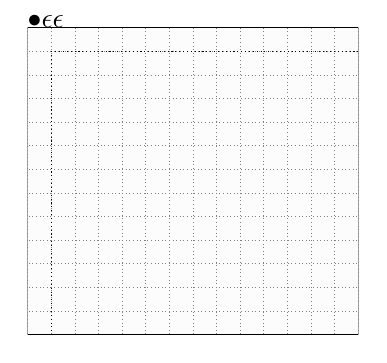
\begin{tikzpicture}[
	xscale=0.3,yscale=-0.3,
    char/.style={draw=none, text centered, anchor=base},
    position/.style={draw=none, text centered, anchor=base}
]

	\begin{pgfscope}
		\pgftransformshift{\pgfpoint{-3cm}{0cm}}
		\clip (3,0) rectangle (17, 13);
		\draw[draw=none,fill=gray!2] (1,0) rectangle (17, 13);
		\draw[style=grid lines](0,0) grid +(20,20);
		\draw[black] (3,0) rectangle (17, 13);
		\draw[black,densely dotted] (4,1) -- (4, 13);
		\draw[black,densely dotted] (4,1) -- (17, 1);
	\end{pgfscope}
	
	\def\CharFont{\scriptsize\sffamily}
	\PrintStringOnly{0}{0.1}{0,1,2,3,4,5,6,7,8,9,10,11,12,13}
	\PrintStringOnly{0}{1.1}{0,1,2,3,4,5,6,7,8,9}
	\PrintStringOnly{0}{2.1}{0,1,2,3,4,5,6,7,8,9}
	\PrintStringOnly{0}{3.1}{0,1,2,3,4,5,6,7,8,9}
	\PrintStringOnly{0}{4.1}{0,1,2,3,4,5,6,7,8,9}
	\PrintStringOnly{0}{5.1}{0,1,2,3,4,5,6,7,8,9}
	\PrintStringOnly{0}{6.1}{0,1,2,3,4,5,6,7,8,$\bullet$}

	\def\CharFont{\small\sffamily}
	\PrintStringOnly{0}{-1.1}{$\epsilon$,C,G,C,A,N,A,T,A,A,T,C,A,G}
	\PrintVStringOnly{-1.2}{0.1}{$\epsilon$,C,G,G,C,A,A,T,A,T,C,A,G}

\end{tikzpicture}

\end{center}
\end{figure}


% === Overview of existing methods ===

\section{String matching}

%\subsection{Problem definition}

We can now define \emph{exact string matching}, perhaps the most fundamental problem in stringology.
Given a string $p$ (with $|p|=m$) called the \emph{pattern} and a longer string $t$ (with $|t|=n$) called the \emph{text}, the exact string matching problem is to find all occurrences, if any, of pattern $p$ into text $t$ \citep{Gusfield1997}.
This problem has been extensively studied from the theoretical standpoint and is well solved in practice.

The definition of distance functions between strings let us generalize exact string matching into a more challenging problem: \emph{approximate string matching}.
Given a text $t$, a pattern $p$, and a \emph{distance threshold} $k \in \N$, the approximate string matching (a.s.m.) problem is to find all occurrences of $p$ into $t$ within distance $k$.
The a.s.m. problem under the Hamming distance is commonly referred as the \emph{$k$-mismatches} problem and under the edit distance as the \emph{$k$-differences} problem.
For $k$-mismatches and $k$-differences, it must hold $k > 0$ as the case $k = 0$ corresponds to exact string matching, and $k < m$ as a pattern occurs at any position in the text if we substitute all its $m$ characters.
Under these distances, we define the \emph{error rate} as $\epsilon = \frac{k}{m}$, with $0 < \epsilon < 1$ given the above conditions, and we alternatively refer to these a.s.m. problems as $\epsilon$-mismatches and $\epsilon$-differences.

We can classify string matching problems in two categories, \emph{online} and \emph{offline}, depending on which string, the pattern or the text, is given first.
Algorithms for online string matching work by preprocessing the pattern and scanning the text from left to right (or right to left); their worst-case runtime complexity ranges from $\Oh(nm)$ to $\Oh(n)$ while their worst-case memory complexity ranges from $\Oh(\sigma^k m^k)$ to $\Oh(m)$.
Algorithms for offline string matching are instead allowed to preprocess the text; their worst-case runtime complexity ranges from $\Oh(m)$ to $\Oh(\sigma^k m^k)$ while their worst-case memory complexity is usually $\Oh(n)$.
In practice, if the text is long, static and searched frequently, offline methods largely outperform online methods in terms of runtime, provided the necessary amount of memory. Therefore, we concentrate on offline algorithms.

We can subdivide algorithms for offline string matching in two categories: \emph{fully-indexed} and \emph{filtering}.
Fully-indexed algorithms work solely on the index of the text, while filtering methods first use the index to discard uninteresting portions of the text and subsequently use an online method to verify narrow areas of the text.
Filtering methods outperform fully-indexed methods for a vast range of inputs\footnote{When the error rate is low.} and are thus very interesting from a practical standpoint. Nonetheless, filtering methods are just opportunistic combinations of online and fully-indexed methods.

In the following of this section we thus give a brief and non-exhaustive overview of the fundamental techniques for online and (both fully-indexed and filtering) offline string matching.
This overview serves as an introduction to the more involved algorithms presented in chapter~\ref{?} and directly used in applications of part~\ref{part:apps}.
For an extensive treatment of the subject, we refer the reader to complete surveys on exact \citep{Faro2013} and approximate \citep{Navarro2001b} online string matching methods, as well as to a succint survey on indexed methods \citep{Navarro2001}.

% --- Online methods ---

\subsection{Online methods}

We consider two classes of algorithms for online string matching, those based on automata and those based on dynamic programming.

\subsubsection{Automata}

Exact search of one pattern. Knuth-Morris-Pratt automaton.

Exact search of multiple patterns. Aho-corasick automaton.

Approximate search of one pattern. Ukkonen automaton.

\subsubsection{Dynamic programming}

The dynamic programming algorithm~\ref{?} to compute the distance of two strings can be easily turned into a string matching algorithm.
Since an occurrence of the pattern can start and end anywhere in the text, a.s.m. consists of computing the edit distance between the pattern and all substrings of the text.
The problem can be thus solved by computing the edit distance between the text and the pattern without penalizing leading and trailing deletions in the text.

We pose $x=p$ and $y=t$ and consider Equation~\ref{eq:dp-min}.
Since an occurrence of the pattern can start anywhere in the text, we change the initialization of the top row $D[0:]$ of the DP matrix according to the condition:
\begin{eqnarray}
d(\epsilon, y_{1..j}) = 0 \text{ for all } 1 \leq j \leq n
\end{eqnarray}
and since an occurrence of the pattern can end anywhere in the text, we check all cells $D[m,j]$ for all $1 \leq j \leq n$ in the bottom row of $D$ for the condition $D[m,j] \leq k$.

\begin{figure}[h]
\begin{center}
\caption[Example of approximate string matching via DP.]{DP table representing the match of $p=...$ in $t=...$.}
\label{fig:asm-dp}
\begin{tikzpicture}[xscale=0.3,yscale=-0.3]
	\tikzstyle{grid lines}=[gray,densely dotted,line width=0.3pt]
	
	% paralelogram and grid
	\begin{pgfscope}
		\pgftransformshift{\pgfpoint{-3cm}{0cm}}
		\clip (3,0) rectangle (19, 13);
		\draw[draw=none,fill=gray!2] (1,0) rectangle (19, 13);
%		\bandedDotPara{0}{0}{11}{19};
		\fill[fill=DPInitColor] (3,0) rectangle (4,12);
		\fill[fill=DPInitColorDark] (3,12) rectangle (4,13);
		\fill[fill=DPInitColor] (3,0) rectangle (19,1);
		\fill[fill=DPRecurseColor] (4,1) rectangle (19,13);
		\fill[fill=DPRecurseColorDark] (4,12) rectangle (19,13);
		\draw[style=grid lines](0,0) grid +(20,20);
		\draw[black] (3,0) rectangle (19, 13);

		\node at (3.5,0.5) {\sf\tiny \color{DPInitValueColor}0};
		\node at (4.5,0.5) {\sf\tiny \color{DPInitValueColor}0};
		\node at (5.5,0.5) {\sf\tiny \color{DPInitValueColor}0};
		\node at (6.5,0.5) {\sf\tiny \color{DPInitValueColor}0};
		\node at (7.5,0.5) {\sf\tiny \color{DPInitValueColor}0};
		\node at (8.5,0.5) {\sf\tiny \color{DPInitValueColor}0};
		\node at (9.5,0.5) {\sf\tiny \color{DPInitValueColor}0};
		\node at (10.5,0.5){\sf\tiny \color{DPInitValueColor}0};
		\node at (3.5,1.5) {\sf\tiny \color{DPInitValueColor}1};
		\node at (3.5,2.5) {\sf\tiny \color{DPInitValueColor}2};
		\node at (3.5,3.5) {\sf\tiny \color{DPInitValueColor}3};
	\end{pgfscope}
	
	\tikzstyle{labelstyle}=[font=\sf\footnotesize,color=NumberColor]
	
	\node[labelstyle] at (.5,14) {0};
	\node[labelstyle] at (15.5,14) {$n$};
%	\draw[-,color=NumberColor] (-0.45,3.5) -- (-0.15,3.5);

	\node[labelstyle] at (-1,.5) {0};
%	\node[labelstyle,color=black] at (-3,3.5) {$\left\lfloor \frac{m-n+k}{2}\right\rfloor$};
	\node[labelstyle] at (-1,12.5) {$m$};

	\draw[grid lines,fill=DPInitColor]        (17,4)   rectangle +(1,1);
	\draw[grid lines,fill=DPRecurseColor]     (17,5.5) rectangle +(1,1);
%	\draw[grid lines,fill=DPRecurseColorDark] (17,7) rectangle +(1,1);
	\draw[draw=none, fill=DPInitColorDark]    (17,7) -- ++(1,0) -- ++(-1,1) -- ++(0,-1) -- cycle;
	\draw[draw=none, fill=DPRecurseColorDark] (18,7) -- ++(0,1) -- ++(-1,0) -- ++(1,-1) -- cycle;
	\draw[grid lines,fill=none]               (17,7) rectangle +(1,1);
%	\draw[grid lines,fill=gray!2]             (17,8.5)   rectangle +(1,1);
	\node[anchor=base west] at (18,4.85) {\sf\footnotesize initial case};
	\node[anchor=base west] at (18,6.35) {\sf\footnotesize recursive case};
	\node[anchor=base west] at (18,7.85) {\sf\footnotesize tracked score};
%	\node[anchor=base west] at (18,9.35) {\sf\footnotesize ignored};

%	\draw[decorate,decoration={brace,mirror,amplitude=7pt},line width=1pt] (2,5.65) -- (13,5.65) node at (7.5,6.4) [below]{\sf\footnotesize $k+1$} ;

\end{tikzpicture}

\end{center}
\end{figure}


%\subsection{DP bit-parallelism}


% --- Indexed methods ---

\subsection{Indexed methods}
\label{sub:introindex}


Indexed methods are more attractive than online methods when several patterns are to be searched in the same static text.
These methods work by building an index of the text beforehand to speed up subsequent searches.
To this intent, we now introduce \emph{suffix tries}, idealized data structures to index texts.
Moreover, we define a set of generic operations to traverse suffix tries in a top-down fashion.
In chapter~\ref{chr:index}, we will consider various data structures replacing suffix tries in practice.
The generic traversal operations here introduced will let us formulate generic algorithms solving string matching problems on any of these data structures.

\subsubsection{Trie}

Consider a collection of strings, \ie an ordered multiset $\S = \{ s^1, s^2, \dots, s^c \}$ of strings over a common alphabet $\Sigma$.
Assume \wlogs each string $s^i \in \S$ to be padded with a \emph{terminator symbol} $\$^i$ not being part of the string alphabet $\Sigma$.
In addition, assume $\$^i <_{lex} \$^j$ for all indices $i,j$ with $i < j < c$.
Note that the terminator symbol is necessary to ensure that no string $s^i$ is a prefix of another string $s^j$.

The trie $\Si$ of the strings collection $\S$ is a lexicographically ordered tree data structure having one node designated as the root and $c$ leaves, denoted as $\Ln_1 \dots \Ln_c$, where leaf $\Ln_i$ points to string $s^i$.
The entering edge of any node of $\Si$ is labeled with a symbol in $\Sigma$, while the entering edge of any leaf of $\Si$ is labeled with a terminator symbol.
Any path from the root to a leaf $\Ln_i$ spells the string $s^i$, including its terminator symbol $\$^i$.
Figure~\ref{fig:trie} illustrates.

\subsubsection{Suffix trie}

We define the suffix trie as the trie of all suffixes of a string.
Given a string $s$ of length $n$, the suffix trie $\Si$ of $s$ has $n$ leaves and leaf $\Ln_i$ points to suffix $s_{i..n}$.
We easily generalize the suffix trie to index string collections.
Given a collection of padded strings $\Sc = \{ s^1, s^2, \dots, s^c \}$, any leaf of the \emph{generalized suffix trie} is labeled with a pair $(i,j)$ where $i$ points to the string $s^i \in \Sc$ and $1 \leq j \leq n^i$ points to one of the $n^i$ suffixes of $s^i$.
Thus each path from the root to a leaf $(i,j)$ spells the suffix $s^i_{j..n^i}$.
Figure~\ref{fig:stree} illustrates.

Note that the suffix trie so defined contains $\Oh(n^2)$ nodes, yet we only consider the suffix trie as an idealized data structure to expose our algorithms.
The optimal data structure to represent in linear space all suffixes of a given string is the \emph{suffix tree} \citep{Morrison1968}.
However, the suffix tree comes with the restriction that internal nodes must have more than one child and with the property that edges can labeled by strings of arbitrary length (see Figure~\ref{fig:stree}).
This latter property slightly complicates the exposition of our string matching algorithms but it does not affect their runtime complexity nor their result.
For this reason, in the following of this manuscript we always consider \wlogs suffix tries instead of suffix trees.
%We remark that all given algorithms can be generalized to work on trees.

\begin{figure}[h]
\caption{Suffix tree and suffix trie for the string ANANAS.}
\label{fig:stree}
\begin{subfigure}{.5\textwidth}
\begin{center}
\begin{tikzpicture}[scale=1.5,font=\sf]

\tikzstyle{level 1}=[sibling distance=14mm, level distance=10mm]
\tikzstyle{level 2}=[sibling distance=8mm, level distance=14mm]
\tikzstyle{level 3}=[sibling distance=8mm, level distance=14mm] 

%\tikzstyle{transparent}=[edge from parent/.style={draw=none}]
%\tikzstyle{el}=[->,thick,color=gray,text=mycolor1high]

\tikzstyle{transparent}=[edge from parent/.style={draw=none}]
\tikzstyle{el}=[->,thick,color=black,text=black]
\tikzstyle{inner}=[circle,draw,color=black,inner sep=1.5pt]

\node[inner](r) {}
child[transparent] {
node[inner](A) {}
child[transparent] {
node[inner](ANA) {}
child[transparent] {
node[leaf](ANANAS) {$1$}
}
child[transparent] {
node[leaf](ANAS) {$3$}
}
}
child[transparent] {
node[leaf](AS) {$5$}
}
}
child[transparent] {
node[inner](NA) {}
child[transparent] {
node[leaf](NANAS) {$2$}
}
child[transparent] {
node[leaf](NAS) {$4$}
}
}
child[transparent] {
node[leaf](S) {$6$}
}
;

\draw[el] (r) -- (A) \labelA{A};
\draw[el] (A) -- (ANA) \labelB{N}{A};
\draw[el] (ANA) -- (ANANAS) \labelD{N}{A}{S}{\$};
\draw[el] (ANA) -- (ANAS) \labelB{S}{\$};
\draw[el] (A) -- (AS) \labelB{S}{\$};
\draw[el] (r) -- (NA) \labelB{N}{A};
\draw[el] (NA) -- (NANAS) \labelD{N}{A}{S}{\$};
\draw[el] (NA) -- (NAS) \labelB{S}{\$};
\draw[el] (r) -- (S) \labelB{S}{\$};

\end{tikzpicture}


\end{center}
\end{subfigure}%
\begin{subfigure}{.5\textwidth}
\begin{center}
\begin{tikzpicture}[scale=1.5,font=\sffamily]

\tikzstyle{level 1}=[sibling distance=12mm, level distance=6mm]
\tikzstyle{level 2}=[sibling distance=6mm, level distance=6mm]
\tikzstyle{level 3}=[sibling distance=6mm, level distance=6mm] 
\tikzstyle{level 4}=[sibling distance=6mm, level distance=6mm] 
\tikzstyle{level 5}=[sibling distance=6mm, level distance=6mm] 
\tikzstyle{level 6}=[sibling distance=6mm, level distance=6mm] 
\tikzstyle{level 7}=[sibling distance=6mm, level distance=6mm] 

%\tikzstyle{transparent}=[edge from parent/.style={draw=none}]
%\tikzstyle{el}=[->,thick,color=gray,text=mycolor1high]

\tikzstyle{transparent}=[edge from parent/.style={draw=none}]
\tikzstyle{el}=[->,thick,color=black,text=black]
\tikzstyle{inner}=[circle,draw,color=black,inner sep=1.5pt]

\node[inner](r) {}
child[transparent] {
node[leaf](D) {$7$}
}
child[transparent] {
node[inner](A) {}
child[transparent] {
node[inner](AN) {}
child[transparent] {
node[inner](ANA) {}
child[transparent] {
node[inner](ANAN) {}
child[transparent] {
node[inner](ANANA) {}
child[transparent] {
node[inner](ANANAS) {}
child[transparent] {
node[leaf](ANANASD) {$1$}
}
}
}
}
child[transparent] {
node[inner](ANAS) {}
child[transparent] {
node[leaf](ANASD) {$3$}
}
}
}
}
child[transparent] {
node[inner](AS) {}
child[transparent] {
node[leaf](ASD) {$5$}
}
}
}
child[transparent] {
node[inner](N) {}
child[transparent] {
node[inner](NA) {}
child[transparent] {
node[inner](NAN) {}
child[transparent] {
node[inner](NANA) {}
child[transparent] {
node[inner](NANAS) {}
child[transparent] {
node[leaf](NANASD) {$2$}
}
}
}
}
child[transparent] {
node[inner](NAS) {}
child[transparent] {
node[leaf](NASD) {$4$}
}
}
}
}
child[transparent] {
node[inner](S) {}
child[transparent] {
node[leaf](SD) {$6$}
}
}
;

\draw[el] (r) -- (D) \labelA{\$};
\draw[el] (r) -- (A) \labelA{A};
\draw[el] (A) -- (AN) \labelA{N};
\draw[el] (AN) -- (ANA) \labelA{A};
\draw[el] (ANA) -- (ANAN) \labelA{N};
\draw[el] (ANAN) -- (ANANA) \labelA{A};
\draw[el] (ANANA) -- (ANANAS) \labelA{S};
\draw[el] (ANANAS) -- (ANANASD) \labelA{\$};
\draw[el] (ANA) -- (ANAS) \labelA{S};
\draw[el] (ANAS) -- (ANASD) \labelA{\$};
\draw[el] (A) -- (AS) \labelA{S};
\draw[el] (AS) -- (ASD) \labelA{\$};

\draw[el] (r) -- (N) \labelA{N};
\draw[el] (N) -- (NA) \labelA{A};
\draw[el] (NA) -- (NAN) \labelA{N};
\draw[el] (NAN) -- (NANA) \labelA{A};
\draw[el] (NANA) -- (NANAS) \labelA{S};
\draw[el] (NANAS) -- (NANASD) \labelA{\$};
\draw[el] (NA) -- (NAS) \labelA{S};
\draw[el] (NAS) -- (NASD) \labelA{\$};
\draw[el] (r) -- (S) \labelA{S};
\draw[el] (S) -- (SD) \labelA{\$};

\end{tikzpicture}

\end{center}
\end{subfigure}
\end{figure}

\subsubsection{Top-down traversal}

We now give a set of generic operations to traverse tries in a top-down fashion.
Given a trie $\Ti$, we define the following operations inspecting any pointed node $\Tn$ of $\Ti$:
\begin{itemize}
\item \textsc{isRoot}($\Tn$) returns true iff the pointed node is the root;
\item \textsc{isLeaf}($\Tn$) returns true iff the pointed node is a leaf;
\item \textsc{depth}($\Tn$) returns the number of edges from the root to $\Tn$;
\item \textsc{label}($\Tn$) returns the symbol labeling the edge entering $\Tn$;
\item \textsc{getOccurrences}($\Tn$) returns the list of positions pointed by leaves below $\Tn$;
\end{itemize}
and the following operations moving from pointed node $\Tn$, and returning true on success and false otherwise:
\begin{itemize}
\item \textsc{goDown}($\Tn$) moves to the lexicographically smallest child of $\Tn$;
\item \textsc{goDown}($\Tn, c$) moves to the child of $\Tn$ whose entering edge is labeled by $c$;
\item \textsc{goRight}($\Tn$) moves to the lexicographically next child of $\Tn$;
\item \textsc{goUp}($\Tn$) moves to the parent node of $\Tn$.
\end{itemize}

Time complexities of the above operations depend on the data structure implementing the trie.
Usually \textsc{label} is $\Oh(1)$, \textsc{goDown} and \textsc{goRight} are $\Oh(1)$ or sublinear in $n$, \textsc{getOccurrences} can be linear in the size of the occurrences, \textsc{goUp} is $\Oh(1)$ but with an additional $\Oh(n)$ space complexity.
In chapter~\ref{chr:index}, we consider various data structures to implement suffix tries, we show how to implement these operations and give their complexities.

\subsubsection{String matching algorithms}

Using the above generic top-down traversal operations we are able to formulate generic string matching algorithms.
Here we formulate the simple algorithm for exact string matching on a suffix trie.
In chapter~\ref{chr:index}, we give analogous algorithms solving $k$-mismatches and $k$-differences by means of a backtracking top-down traversal \citep{Ukkonen1993, Baeza1999}.

We assume the text $t$ to be indexed by its suffix trie $\Ti$.
Algorithm~\ref{alg:st-exact} searches a pattern $p$ by starting in the root node of $\Ti$ and following the path spelling the pattern.
If the search ends up in a node $\Tn$, each leaf $\Ln_i$ below $\Tn$ points to a distinct suffix $t_{i..n}$ such that $t_{i..i+m}$ equals $p$.
%Algorithm~\ref{alg:st-exact} is correct since each path from the root to any internal node of the suffix trie $\Ti$ spells a different unique substring of $t$; consequently all equal substrings of $t$ are represented by a single common path.
If we implement \textsc{goDown} in constant time and \textsc{getOccurrences} in linear time, we find all occurrences of $p$ into $t$ in optimal time $\Oh(m+o)$, where $m$ is the length of $p$ and $o$ its number of occurrences in $t$.

\begin{algorithm}[h]
\caption{Exact string matching on a suffix trie.}
\label{alg:st-exact}
\begin{algorithmic}[1]
\Procedure{ExactSearch}{$t,p$}
	\If {\Call{atEnd}{$p$}}
		\State \Report \Call{getOccurrences}{$t$}
	\Else
		\State {\Call{goNext}{$p$}}
		\If {\Call{goDown}{$t,\Call{value}{p}$}}
			\State \Call{ExactSearch}{$t,p$}
		\EndIf
	\EndIf
\EndProcedure
\end{algorithmic}
\end{algorithm}

\begin{figure}[h]
\begin{center}
\caption[Exact string matching on a suffix tree.]{Exact string matching on a suffix tree. The pattern NA is searched exactly in the text ANANAS.}
\label{fig:st-exact}
\begin{tikzpicture}[scale=1.5,font=\sf]

\tikzstyle{level 1}=[sibling distance=20mm, level distance=6mm]
\tikzstyle{level 2}=[sibling distance=8mm, level distance=6mm]
\tikzstyle{level 3}=[sibling distance=8mm, level distance=6mm] 
\tikzstyle{level 4}=[sibling distance=5mm, level distance=6mm]

%\tikzstyle{transparent}=[edge from parent/.style={draw=none}]
%\tikzstyle{el}=[->,thick,color=gray,text=mycolor1high]

\tikzstyle{transparent}=[edge from parent/.style={draw=none}]
\tikzstyle{el}=[->,thick,color=black,text=black]
\tikzstyle{inner}=[circle,draw,color=black,inner sep=1.5pt]

\node[inner](r) {}
child[transparent] {
node[inner](G) {}
child[transparent] {
node[inner](GG) {}
child[transparent] {
node[leaf](GGC) {$12$}
}
child[transparent] {
node[inner](GGG) {}
child[transparent] {
node[leaf](GGGC) {$11$}
}
}
child[transparent] {
node[inner](GGT) {}
child[transparent] {
node[leaf](GGTA) {$0$}
}
child[transparent] {
node[leaf](GGTG) {$6$}
}
}
}
}
;

\draw[el] (r) -- (G) \labelA{G};
\draw[el] (G) -- (GG) \labelA{G};

\draw[el] (GG) -- (GGC) \labelA{C};
\draw[el] (GG) -- (GGG) \labelA{G};
\draw[el] (GGG) -- (GGGC) \labelA{C};
\draw[el] (GG) -- (GGT) \labelA{T};
\draw[el] (GGT) -- (GGTA) \labelA{A};
\draw[el] (GGT) -- (GGTG) \labelA{G};

\end{tikzpicture}


\end{center}
\end{figure}


% --- Filtering methods ---

\subsection{Filtering methods}
\label{sec:intro:filtering}

The goal of filtering methods is to obtain algorithms that have favorable average running times.
The principle under which they work is that large and uninteresting portions of the text can be quickly discarded, while narrow and highly similar portions can be verified with a conventional online method.
We remark that any filtering method can either work in a online fashion or take advantage of an index of the text to speed up the filtration phase.
Here we always consider the filtration phase to be indexed.

Filtering methods work under the assumption that given patterns occur in the text with a \emph{low average probability}.
Such probability is a function of the error rate $\epsilon$, in addition to the alphabet size $\sigma$, and can be computed or estimated under the assumption of the text being generated by a specific random source.
Under the uniform Bernoulli model, where each symbol of $\Sigma$ occurs with probability $\frac{1}{\sigma}$, \citet{Navarro2000} estimates that $\epsilon < 1 - \frac{1}{\sigma}$ is a conservative bound on the error rate which ensures few matches, and for which filtering algorithms are effective.
For higher error rates, non-filtering online and indexed methods work better.

We call a filter \emph{lossless} or \emph{full-sensitive} if it guarantees not to discard any occurrence of the pattern, otherwise we call it \emph{lossy}.
Lossy filters can be designed to solve approximately $\epsilon$-differences.
We focus our attention on lossless filters. 

We now consider two classes of filtering methods: those based on \emph{seeds} and those based on \emph{$q$-grams}.
Filters based on seeds partition the pattern into \emph{non-overlapping} factors called seeds.
We can derive full-sensitive partitioning strategies by application of the pigeonhole principle.
Instead, filters based on $q$-grams consider all \emph{overlapping} substrings of the pattern having length $q$, the so-called $q$-grams.
Eventually, simple lemmas gives us lower bounds on the number of $q$-grams that must be present in a narrow window of the text as necessary condition for an occurrence of the pattern.

\subsubsection{Seed filters}

We start by considering the case of two arbitrary strings $x,y$ \st $d_E(x,y) \leq k$.
If we partition \wlogs $y$ into $k+1$ non-overlapping seeds, then at least one seed will occur as a factor of $x$.
\begin{lemma}
\label{lemma:exact-seeds}
\citep{Baeza1999b}
Let $x,y$ be two strings \st $d_E(x,y) = k$ for some $k \in \N_0$.
If $y=y^1 y^2 \dots y^{k+1}$ then $x=ay^ib$ for some $a, b$.
\end{lemma}
\begin{proof}
We proceed by induction on $k$.
For $k=0$, the string $y$ is partitioned into only one factor, $y$ itself.
The condition $d_E(x,y) = 0$ implies $x=y$, which is true for $a=\epsilon$ and $b=\epsilon$.
We suppose the case $k=j-1$ to be true, thus since $d_E(x,y) = j-1$ and $y=y^1 y^2 \dots y^{j}$ then $x=ay^ib$ for some $a, b$.
We consider the case $k=j$. The $j$-th error can be in
\begin{inparaenum}[(i)]
\item\label{lemma:exact-seeds:prefix} $y^1\dots y^{i-1}$,
\item\label{lemma:exact-seeds:infix} $y^i$, or
\item\label{lemma:exact-seeds:suffix} $y^{i+1}\dots y^{j}$.
\end{inparaenum}
In case~\ref{lemma:exact-seeds:prefix} or~\ref{lemma:exact-seeds:suffix}, $x=ay^ib$ clearly holds.
In case~\ref{lemma:exact-seeds:infix}, if we partition $y^i$ in two factors $y^{i'}$ and $y^{i''}$, then either $x=ay^{i'}b'$ or $x={a'}y^{i''}b$.
\end{proof}

Thus, we solve $k$-differences by partitioning the pattern into $k+1$ seeds and searching all seeds into the text, \eg with the help of a substring index.
Figure~\ref{fig:seeds-ext} shows an example.
Note that we are reducing one approximate search into many smaller exact searches.
As Lemma~\ref{lemma:exact-seeds} gives us a necessary but not sufficient condition, we must verify whether any candidate location induced by an occurrence of some seed corresponds to an approximate occurrence of the pattern in the text.
Thus, we verify any substring $s$ of the text of length $m - k \leq |s| \leq m + k$ containing one seed of $p$.

\begin{figure}[h]
\begin{center}
\caption{Filtration with exact seeds.}
\label{fig:seeds-ext}
\begin{tikzpicture}[font=\normalsize\sffamily]

\transcript{25}{G/M/G, C/M/C, T/M/T, N/R/A, T/M/T, G/M/G, G/D/$-$, G/M/G, C/M/C, A/M/A, T/M/T, T/M/T, A/R/G, T/M/T, G/M/G, G/M/G, C/M/C, $-$/I/C, C/M/C, A/M/A, T/M/T, T/M/T, T/M/T, T/R/A, T/M/T}{1}
\band{25}
\seed{1}{25}{1}

\node[left=0.25cm of read_1] {$p$} ;
\node[left=0.25cm of genome_1] {$t$} ;

% Unaffected seeds
\foreach \x in {9}
{
	\qgramo{\x}{$\#$, $\#$, $\#$, $\#$}{1}{1}
}

% Covered seeds
\foreach \x in {1,5,13,22}
{
	\qgramo{\x}{$\#$, $\#$, $\#$, $\#$}{1}{0}
}
\qgrami{17}{$\#$, $ $, $\#$, $\#$, $\#$}{1}

% Strikes over covered seeds
\draw[strike] (qgram_1_4.north) -- (qgram_1_4.south) ;
\draw[strike] (qgram_5_3.north) -- (qgram_5_3.south) ;
\draw[strike] (qgram_13_1.north) -- (qgram_13_1.south) ;
\draw[strike] (qgram_22_3.north) -- (qgram_22_3.south) ;

\end{tikzpicture}
\end{center}
\end{figure}

How many verifications we expect to have?
\begin{eqnarray}
p_\alpha = \frac{1}{\sigma} \text{ for all } \alpha \in \Sigma\\
\text{Pr}(H > 0) = \frac{1}{\sigma^q}\\
E(H) = \sum_{i=1}^{n-q+1}{\text{Pr}(H > 0)} = \frac{n - q + 1}{\sigma^q} \leq \frac{n}{\sigma^q}\\
E(V) = (k + 1) \cdot E(H) < \frac{n (k + 1)}{\sigma^q}
\end{eqnarray}

Which is the runtime of the algorithm?

How to choose the partitioning? Which length of $q$ makes filtration lossless?
$q=\left \lfloor \frac{m}{k+1} \right \rfloor$.


\subsubsection{$q$-Gram filters}

$q$-Gram filters are based on the so-called $q$-gram similarity measure $\tau_q : \Sigma^{*} \times \Sigma^{*} \rightarrow \N_0$, defined as the number of substrings of length $q$ common to two given strings.
The following lemma relates $q$-gram similarity to edit distance\footnote{Thus it relates $q$-gram similarity also to Hamming distance.}.
It gives a lower bound on the $q$-gram similarity $\tau_q(x,y)$ for any two strings $x,y$ for which $d_E(x,y) = k$.
This means that $\tau_q(x,y) \geq k$ is a necessary but not sufficient condition for $d_E(x,y) \leq k$.
\begin{lemma}
\label{lemma:qgrams}
\citep{?}
Let $x,y$ be two strings with edit distance $k$ and $\min\{|x|,|y|\} = m$, then $x$ and $y$ have $q$-gram similarity $\tau_q(m,k) \geq m - q + 1 - kq$.
\end{lemma}
\begin{proof}
By induction on k.
\end{proof}

Note how the threshold depends on $q$ and $(m,k)$.

How can we use this result to solve approximate string matching?
The lemma itself does not give us the direct solution, indeed it considers the edit distance between two arbitrary strings, while in a.s.m. the pattern can match any substring of the text.
In the case of Hamming distance, if the pattern matches any substring $s$ of $t$, then $s$ must have length $m$.
In the case of edit distance, it must hold $m - k \leq |s| \leq m + k$.
The dot-plot representation helps us to visualize this concept.
Hamming distance occurrences cover one single diagonal of the dot-plot, while edit distance occurrences are enclosed inside a parallelogram of side $2k+1$.

Overlapping parallelograms?

We can design a filtration algorithm that scans the text and counts how many $q$-grams of the pattern falls into each parallelograms.
Only the parallelograms exceeding the threshold $\tau_q(m,k)$ have to be verified with an online method, \eg standard DP.
To speed up the filtration phase, the $q$-grams can be counted with the help of a substring index.

Which length of $q$ makes filtration lossless? $q=\left \lfloor \frac{m}{k+1} \right \rfloor$.

\begin{figure}[h]
\begin{center}
\caption{Filtration with $q$-grams.}
\label{fig:qgrams-ext}
\begin{tikzpicture}[font=\normalsize]

\transcript{25}{G/M/G, C/M/C, T/M/T, N/R/A, T/M/T, G/M/G, G/M/G, G/D/$ $, C/M/C, A/M/A, T/M/T, A/R/G, T/M/T, T/M/T, G/M/G, A/R/G, G/M/C, C/M/C, C/M/C, G/R/A, T/M/T, T/M/T, T/M/T, A/M/A, T/M/T}{4}
\band{25}
\seed{1}{25}{1}

\node[left=0.25cm of read_1] {$p$} ;
\node[left=0.25cm of genome_1] {$t$} ;

\foreach \x in {1,...,22}
{
	\pgfmathtruncatemacro{\y}{1+Mod(\x-1,4)}
	\qgram{\x}{$\#$, $\#$, $\#$, $\#$}{\y}
}

\draw[line] (read_1.south)+(0,-1*0.4) -- (transcript_1);
\draw[line] (read_2.south)+(0,-2*0.4) -- (transcript_2);
\draw[line] (read_3.south)+(0,-3*0.4) -- (transcript_3);

\draw[line] (qgram_20_4.north) -- (qgram_22_2);
\draw[line] (read_24.south)+(0,-2*0.4) -- (transcript_24);
\draw[line] (read_25.south)+(0,-2*0.4) -- (transcript_25);
\draw[line] (qgram_22_4.north) -- (read_25.south);

\foreach \x in {1,...,20}
{
	\pgfmathtruncatemacro{\y}{4-Mod(\x-1,4)}
	\draw[strike] (qgram_\x_\y.north) -- (qgram_\x_\y.south) ;
}

\end{tikzpicture}
\end{center}
\end{figure}
